% all-in-one cheatsheet layout (Michael Franzen, 2013)
\documentclass[a4paper]{article}

% geometry settings
\usepackage[top=2cm, bottom=2.5cm, left=2cm, right=2cm]{geometry}

% font settings
%\usepackage[light,math]{kurier}
\usepackage[T1]{fontenc}
\usepackage[utf8]{inputenc}
\usepackage{marvosym}
\usepackage{amssymb}
\usepackage{amsfonts}
\usepackage{amsmath}
\usepackage{amsthm}

% colors
\usepackage{xcolor}
\definecolor{lightgray}{gray}{0.8}

% formatting
\usepackage{paralist}
\usepackage{multicol}
\usepackage{tabularx}
\usepackage{Tabbing}
\usepackage{booktabs}
\usepackage{fancyhdr}
\usepackage{url}
\usepackage[framemethod=tikz]{mdframed}
\pagestyle{fancy}

% math
\usepackage{array}
\usepackage{eqnarray}
\usepackage{mathtools}
\usepackage{cases}

% figures
\usepackage{wrapfig}
\usepackage{subfigure}

% figure modules
\usepackage{graphicx}
\usepackage{tikz}
\usetikzlibrary{positioning,calc, shapes}
\usepackage{algorithm2e}
\usepackage{verbatim}	

% TOC & Glossary
\usepackage{sectsty}
\usepackage[nottoc,notlof,notlot]{tocbibind}
\usepackage[titles,subfigure]{tocloft}

% commands
\usepackage{xargs}
\usepackage{ifthen}

% head line
\fancyhf{}
\chead{Graph Theory - Sheet 6 - \today\\J. Batzill (1698622), M. Franzen (1696933), J. Labeit (1656460)}
\renewcommand{\headrulewidth}{0.4pt} %obere Trennlinie

\newcommand{\sheetnumber}{1}

% (problem number)
\surroundwithmdframed[
    hidealllines=true,
    backgroundcolor=gray!10,
    skipbelow=\baselineskip,
    skipabove=\baselineskip
]{mylemma}

\surroundwithmdframed[
	linecolor=white,
	skipbelow=\baselineskip,
	skipabove=\baselineskip
]{mytheorem}

\tikzstyle{nod}= [circle, draw,inner sep=0pt, minimum size=0.5cm] 

\begin{document}
	
	\newtheorem{mytheorem}{Theorem}[section]
	\newtheorem{mylemma}{Lemma}[mytheorem]	

	\newenvironmentx*{solution}[1]{\section*{Problem #1}\addtocounter{section}{1}\setcounter{mylemma}{0}\setcounter{mytheorem}{0}}{}
	\newenvironmentx*{theorem}[1]{\begin{mytheorem}#1\begin{proof}}{\end{proof}\end{mytheorem}}
	\newenvironmentx*{lemma}[1]{\begin{mylemma}#1\begin{proof}}{\end{proof}\end{mylemma}}


	\begin{solution}{21}
		\begin{lemma}{In every planar triangulation $G$ on atleast four vertices, there exists a vertex $v$ which does not lie on the outer bound of $G$}
		For the sake of contradiction let's assume there is no such vertex $v$. 
		Then all the vertices lie on the outer bound of $G$ forming a cycle with atleast four vertices. 
		This is a contradiction with $G$ being a planar triangulation, because we can add a edge between two not adjacent vertices to $G$ and the result is still planar. 
		Hence, there has to be atleast one vertex $v$ not on the outer bound of $G$. 
		\end{lemma}
	
		\begin{theorem}{Every planar triangulation $G$ on atleast four vertices contains a vertex whose neighbourhood induces a cycle.}
		After lemma 1.0.1 there exists a vertex $v$ which does not lie on the outer bound of $G$. 
		Let $N(v) = {p_1,p_2,...,p_n}$ be the neighbourhood of $v$. 
		$N(v)$ induces a cycle if all $p_i$ are connected to a cycle and if there are no additionally edges between $p_i$ and $p_j$ with $|i-j|>1$.  
		We first will proof that all $p_i$ form a cycle, hence the induced subgraph $N(v)$ has a cycle as a subgraph. 
		For the sake of contradiction let's assume this is not the case, hence there is $p_i$ and $p_{i+1}$ which are not connected. 
		This is either a contradiction with $v$ not lying on the outer bound of $G$, or with $G$ being a maximal planar graph. 
		Because if $v_i$ and $v_{i+1}$ are not connected and $v$ is not on the outer bound of $G$ there is a face bounded by $v$,$p_i$,$p_{i+1}$ and atleast one additional vertex. 
		This face could be again divided into to smaller faces by adding an edge, hence $G$ is no triangulation. 
		Now we will proof that either $N(v)$ has no additional edges and thus is a cycle or that one of the vertices adjacent to $v$ induces a cycle. 
		\begin{itemize}
			\item \emph{There are no additional edges connecting two vertices $p_i$ and $p_j$ with $|i-j|>1$.} \\
				In this case $N(v)$ is a cycle and we found a vertex whose neighbourhood induces a cycle.
			\item \emph{There is an edge $p_ip_{i+2}$}\\
				In this case the neighbourhood induces graph of $p_{i+1}$ is a cycle namely $p_i p_{i+1} v$. 
			\item \emph{There is an edge between to vertices $p_i$ and $p_j$ with $|i-j| > 2$  and without loss of generality $i<v$.}\\
				This case there is a bounded face in $G$ which is not a triangle. 
				This face is the face bounded by at least the edges $p_ip_{i+1}$, $p_j p_{j-1}$, $p_i p_j$ and atleast one or more edges forming a path from $p_{i+1}$ to $p_{j-1}$. 
				Hence this case can never occur in a planar triangulation. 
		\end{itemize} 
		 In summary we now that we can always find a vertex $v$ whose neighbourhood induces a cycle or one of the neighbours of $v$ here called $p_{i+1}$ has a neighbourhood inducing a cycle.  
		\end{theorem}
		
		\begin{lemma}{Every planar graph $G$ with a maximal number of triangles and atleast 4 vertices has a vertex of degree 3.}
		Using theorem 1.1 we can find a vertex $v$ whose neighbourhood induces a cycle $p_1 p_2 ... p_n$. 
		In the following we will show by induction over the degree of $v$ that if $G$ has a maximal number of triangles, $v$ cannot have a degree greater than $3$. 
		\paragraph{Basis: $v$ has a degree of 4}
		If $v$ has a degree 4, then the subgraph with the nodes $v,p_1,p_2,p_3,p_4$ only has 4 triangles.
		We can change the edge set of this subgraph to get a subgraph with the same vertices and the same outer structure but with containing 6 triangles. 
		We can achieve this by removing edge $v p_3$ and adding the edge $p_2 p_4$. 
		Thus we know that if $G$ has a maximal number of triangles $v$ cannot have degree 4. 
		\begin{center}
			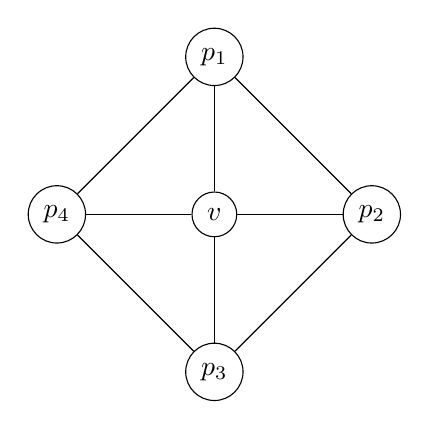
\begin{tikzpicture}
				\node[circle, draw] (v) at (0, 0) {$v$};
				\node[circle, draw] (p1) at (0, 2) {$p_1$};
				\node[circle, draw] (p2) at (2, 0) {$p_2$};
				\node[circle, draw] (p3) at (0, -2) {$p_3$};
				\node[circle, draw] (p4) at (-2, 0) {$p_4$};
				\draw(v) -- (p1);
				\draw(v) -- (p2);
				\draw(v) -- (p3);
				\draw(v) -- (p4);
				\draw(p1) -- (p2);
				\draw(p2) -- (p3);
				\draw(p3) -- (p4);
				\draw(p4) -- (p1);
			\end{tikzpicture}
			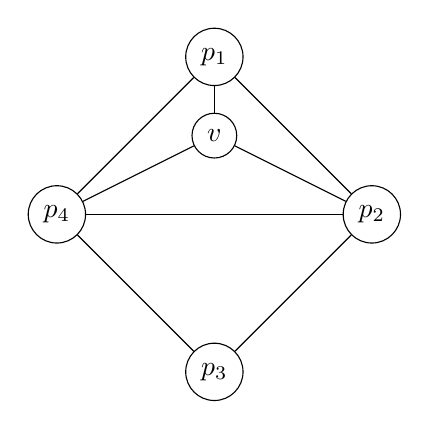
\begin{tikzpicture}
				\node[circle, draw] (v) at (0, 1) {$v$};
				\node[circle, draw] (p1) at (0, 2) {$p_1$};
				\node[circle, draw] (p2) at (2, 0) {$p_2$};
				\node[circle, draw] (p3) at (0, -2) {$p_3$};
				\node[circle, draw] (p4) at (-2, 0) {$p_4$};
				\draw(v) -- (p1);
				\draw(v) -- (p2);
				\draw(v) -- (p4);
				\draw(p1) -- (p2);
				\draw(p2) -- (p3);
				\draw(p3) -- (p4);
				\draw(p4) -- (p1);
				\draw(p4) -- (p2);
			\end{tikzpicture}
		\end{center}
		
		\paragraph{Induction step}
		Let the degree of $v$ be $n>3$. 
		We now can again change the edges set without changing the outer structure of the induced subgraph $N(v)$ so that $v$ has degree $n-1$ and the number of triangles in $N(v)$ stays the same. 
		We can achieve this by removing the edge $v p_2$ and adding the edge $p_1 p_3$. 
		By induction we can repeat this operation until $n=4$ and have the base case. 
		Thus we can increase the number of triangles in the subgraph without changing the vertex count or the outer structure. 
		Hence, the degree of $v$ cannot be greater than 3 if $G$ has a maximal number of triangles.
		\begin{center}
			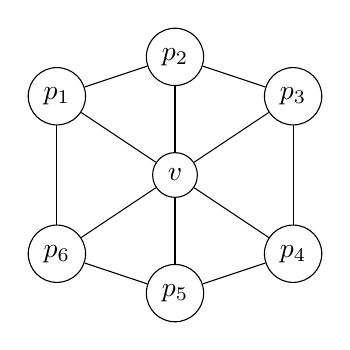
\begin{tikzpicture}
				\node[circle, draw] (v) at (0, 0) {$v$};
				\node[circle, draw] (p1) at (-1.5, 1) {$p_1$};
				\node[circle, draw] (p2) at (0, 1.5) {$p_2$};
				\node[circle, draw] (p3) at (1.5, 1) {$p_3$};
				\node[circle, draw] (p4) at (1.5, -1) {$p_4$};
				\node[circle, draw] (p5) at (0, -1.5) {$p_5$};
				\node[circle, draw] (p6) at (-1.5, -1) {$p_6$};
				\draw(v) -- (p1);
				\draw(v) -- (p2);
				\draw(v) -- (p3);
				\draw(v) -- (p4);
				\draw(v) -- (p5);
				\draw(v) -- (p6);
				\draw(p1) -- (p2);
				\draw(p2) -- (p3);
				\draw(p3) -- (p4);
				\draw(p4) -- (p5);
				\draw(p5) -- (p6);
				\draw(p6) -- (p1);
			\end{tikzpicture}
						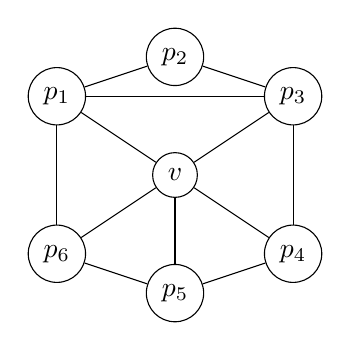
\begin{tikzpicture}
				\node[circle, draw] (v) at (0, 0) {$v$};
				\node[circle, draw] (p1) at (-1.5, 1) {$p_1$};
				\node[circle, draw] (p2) at (0, 1.5) {$p_2$};
				\node[circle, draw] (p3) at (1.5, 1) {$p_3$};
				\node[circle, draw] (p4) at (1.5, -1) {$p_4$};
				\node[circle, draw] (p5) at (0, -1.5) {$p_5$};
				\node[circle, draw] (p6) at (-1.5, -1) {$p_6$};
				\draw(v) -- (p1);
				\draw(v) -- (p3);
				\draw(v) -- (p4);
				\draw(v) -- (p5);
				\draw(v) -- (p6);
				\draw(p1) -- (p2);
				\draw(p2) -- (p3);
				\draw(p3) -- (p4);
				\draw(p4) -- (p5);
				\draw(p5) -- (p6);
				\draw(p6) -- (p1);
				\draw(p1) -- (p3);
			\end{tikzpicture}
		\end{center}
		
		\end{lemma}
		
		
		\begin{theorem}{Every $n$-vertex planar graph has at most $3n-8$ triangles.}
		Let $G$ be a planar graph with a maximal number of triangles. 
		In the following we will show by induction that a planar graph $G$ with atleast 3 vertices with a maximum number of triangles has exactly $3n-8$ triangles. 
		\paragraph{Base: $n=3$}
		The planar graph with maximum number of triangles is $K3$ which has one triangle. 
		$3n-8 = 3*3-8 = 1$ so for the base case the formula is correct.  
		\paragraph{Induction Step}
		Let $G$ be such a graph with $n$ nodes. 
		By using lemma 1.1.1 we can find a vertex $v$ with degree 3 whose neighbourhood induces a cycle.
		If we remove this node we decrease the number of nodes by one and the number of triangles by 3. 
		By induction we know that the resulting graph has no more than $3*(n-1) -8$ triangles. 
		Hence, we know that $G$ has no more than $3*(n-1) -8 + 3 = 3*n-8$ triangles. 
		\end{theorem}
	\end{solution}
	\newpage
	\begin{solution}{22}
		\begin{theorem}{Any $TK_3$-free graph $G$ on $n$ vertices contains a maximum of $n-1$ edges.}
			First, $K_3$ is the triangle $C_3$. Subdividing any edge of $C_i$ results in $C_{i+1}$. Moreover, any cycle has a $TC_3 = TK_3$.
			
			Hence, a graph $G$ is $TK_3$-free if and only if it is acyclic. Further we assume that $G$ is connected (since joining two disjoint acyclic components will not create a cycle but increase the edge count).\\

			From these considerations, the maximum number of edges of an $n$-vertex, $TK_3$-free graph equals the maximum number of edges in an $n$-vertex tree. Any $n$-vertex tree contains a maximum of $n - 1$ edges.
		\end{theorem}

		\begin{theorem}{If a graph $G$ is $3$-connected then $TK_4 \subseteq G$.}
			By \textsc{Tutte (1961)}, any $3$-connected graph has a construction sequence $G_0, G_1, ..., G_n$ whereby $G_0 = K_4$ and $G_n = G$.

			For any $i < n$, $G_i = (V_i, E_i)$ can be constructed by contracting an edge $e = \{x, y\}$ of $G_{i+1}$ ($x, y \in V_{i+1}$, $d(x), d(y) \geq 3$).

			Since $d(y) \geq 3$ and contracting $e$ results in $G_i$, we can effectly say that there is a third vertex $z$ in $G_i$ which is also in $G_{i+1}$ for which $\{\{x,y\}, \{y, z\}\}$ is a subdivision of $\{x,z\}$.

			Thus, $G_{i+1}$ has a $TG_{i}$ and inductively, by the transitivity of topological minority, $G_{i+1}$ has a $TG_0 = TK_4$.
		\end{theorem}
	\end{solution}
	
\end{document}
